\chapter{Funkce PROTOPlantu, aneb „Co to všechno umí?“}
V~této kapitole se pokusím rozebrat funkce řídící jednotky a~dalších přídavných modulů.
Jednotlivé funkce jsou přehledně vyobrazeny na schématech \ref{fig:FEATURES_WHOLE_SMALL} a~\ref{fig:add-MODULES}.
Mezi nejdůležitější funkce PROTOPlantu patří:
\begin{itemize}
    \item možnost řízení ventilace pomocí otevírání oken, nebo ventilátorů
    \item řízení zavlažování
    \item měření teploty a~vlhkosti vzduchu
    \item měření vlhkosti půdy
    \item možnost vytápění
    \item podpora Wi-Fi -- možnost sledování stavu skleníku přes internet, nebo pomocí mobilní aplikace (funkce zatím ve vývoji)
    \item možnost přidání funkce řízení osvětlení
\end{itemize}

\begin{figure}[htbp]
    \centering
    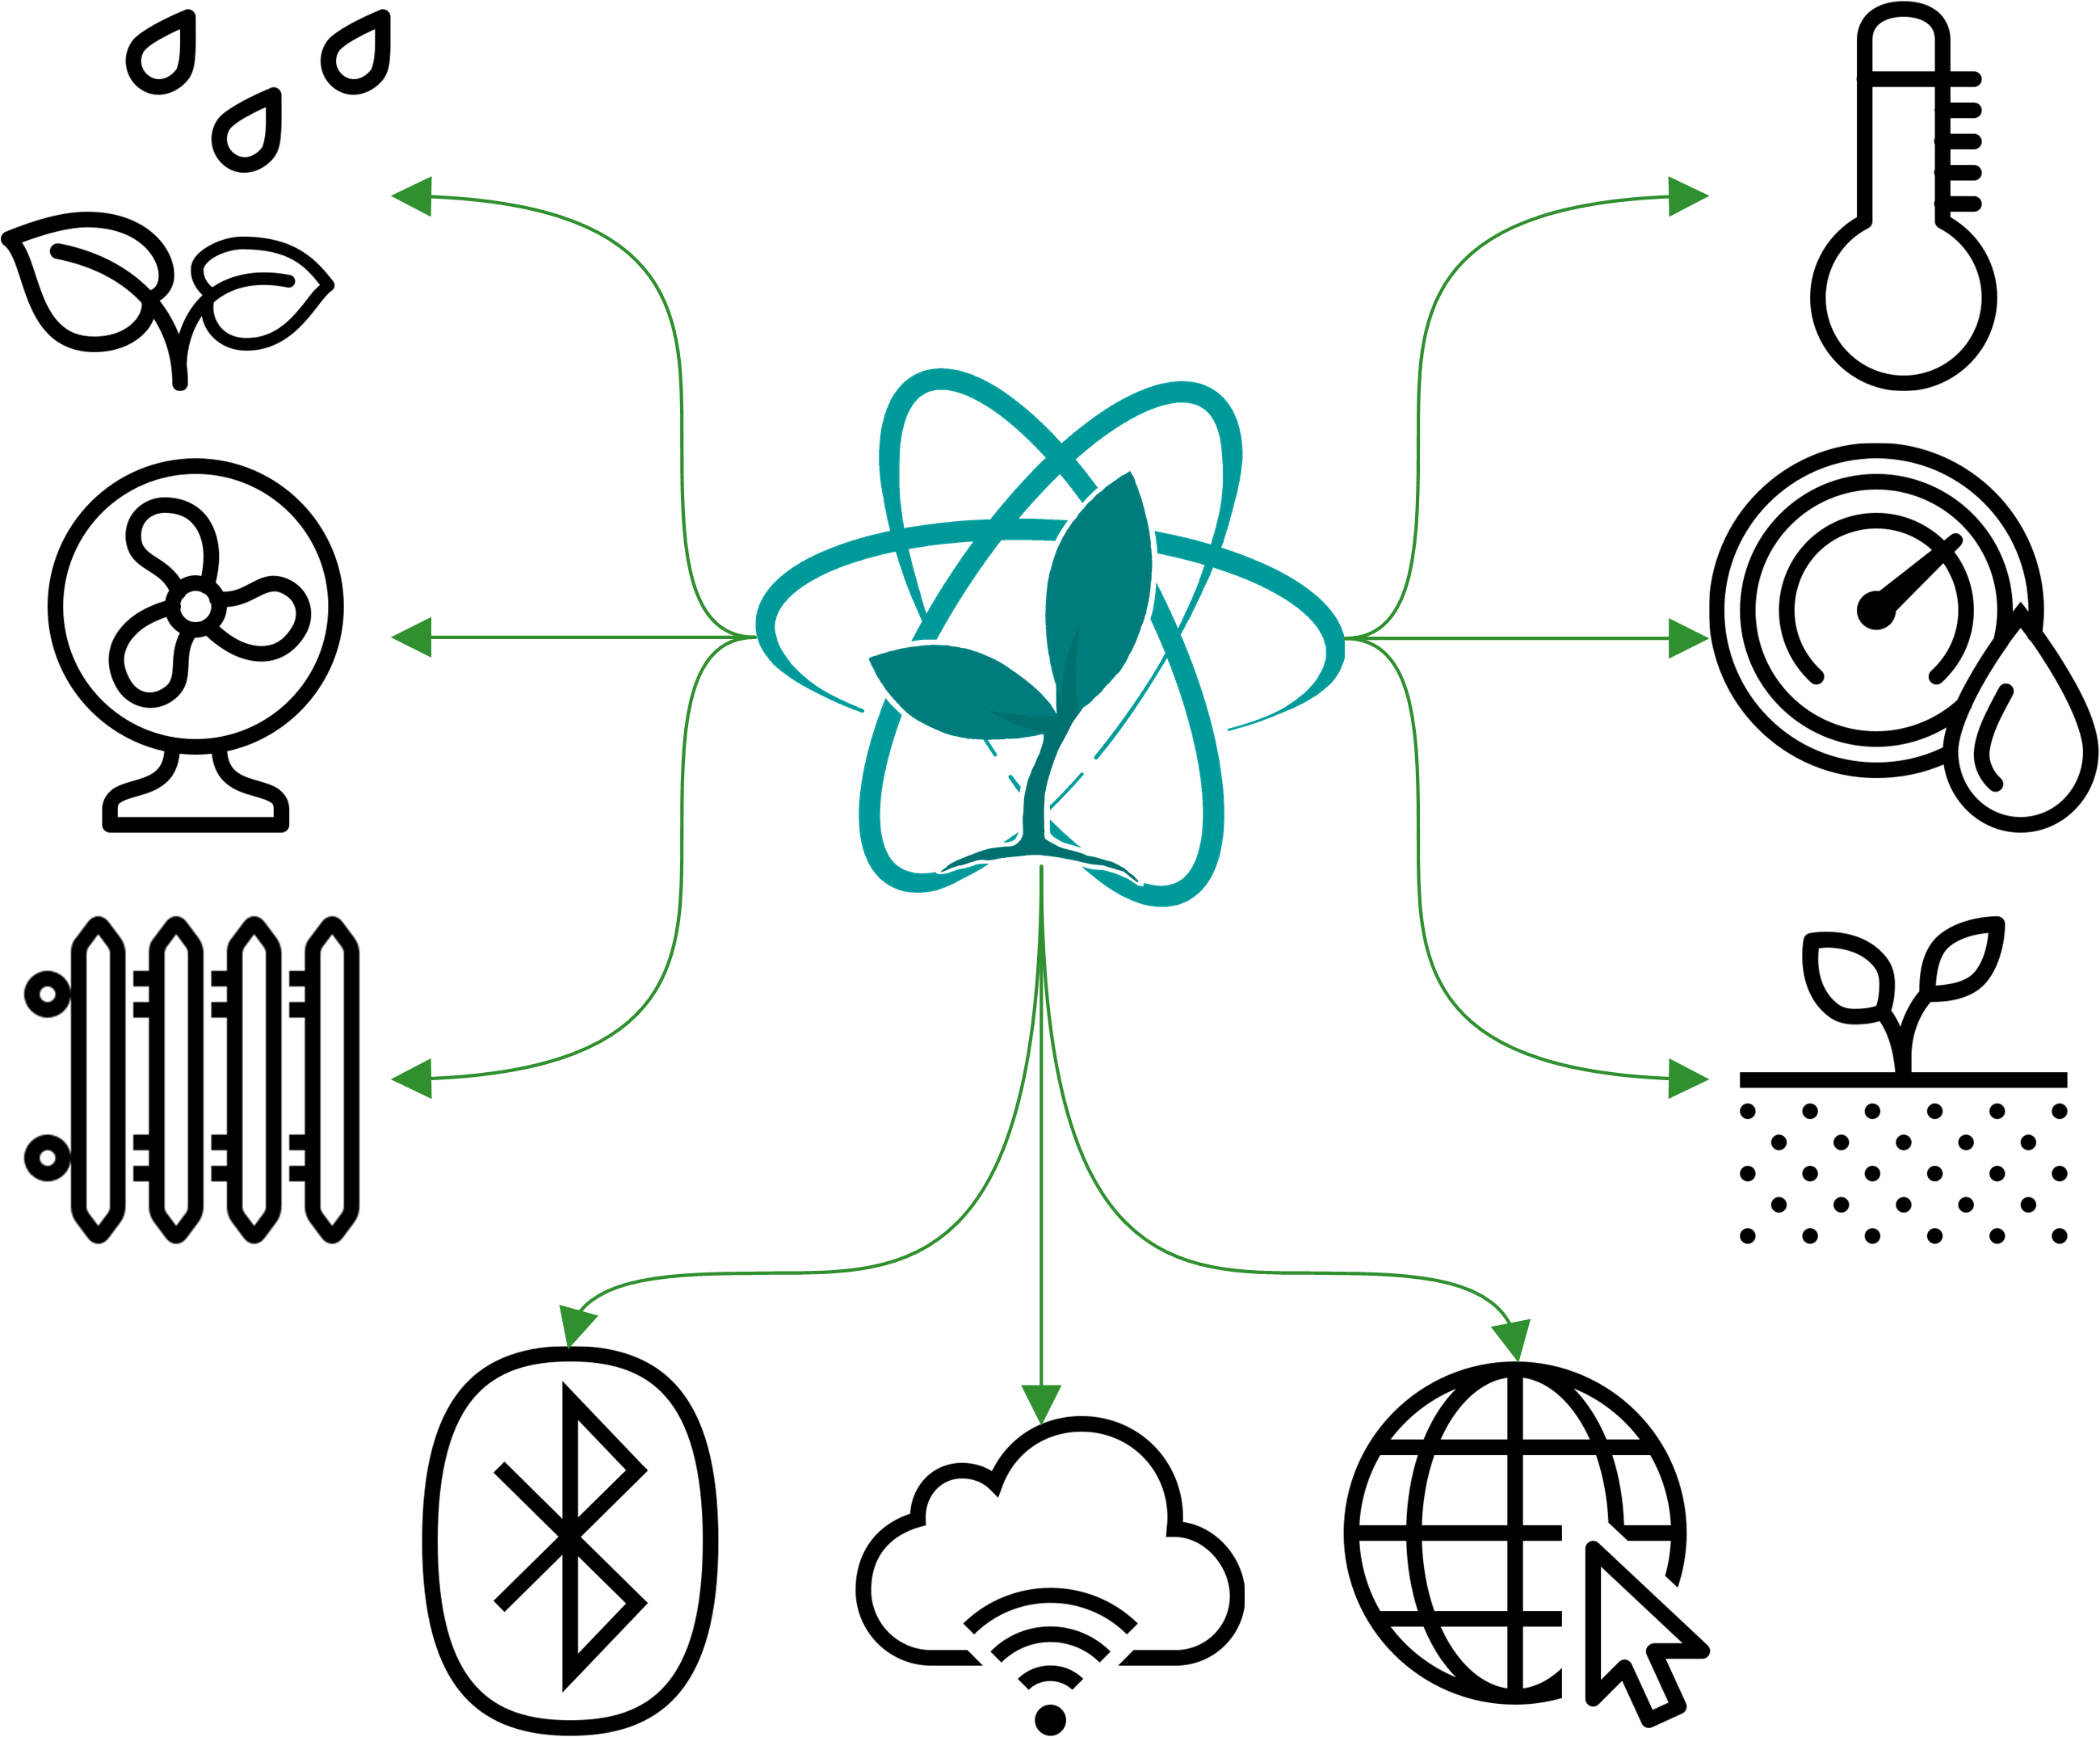
\includegraphics[scale=0.9]{img/FUNCTIONS/PROTOPLANT_FC.png}
    \caption{Zjednodušený diagram funkcí PROTOPlantu.}
    \label{fig:FEATURES_WHOLE_SMALL}
\end{figure}

\section{Funkce řídící jednotky}
Řídící jednotka, neboli PPCU je zároveň i základním modulem celého systému.
Sama o~sobě je schopna vykonávat spoustu funkcí.
Její schopnosti se pak dají ještě více rozšířit dalšími moduly.
Mezi nejdůležitější funkce patří:
\begin{itemize}
    \item dva víceúčelové výstupy pro připojení např. čerpadel, aktuátorů ovláda\-jí\-cích okna, ventilátorů a~jiných spotřebičů
    \item možnost připojení až 30-ti senzorů pro měření teploty (viz kapitola \ref{sec:DS18B20})
    \item 6 volných víceúčelových pinů pro připojení jakýchkoliv dalších periferií (senzory půdní vlhkosti, řízení osvětlení atp.)
    \item možnost připojení k~internetu
    \item LCD displej pro zobrazování naměřených hodnot
\end{itemize}

\section{Funkce dalších modulů}
Jak jsem již zmínil, s~pomocí přídavných modulů se dají funkce PPCU ještě více rozšířit.
Nutno ovšem poznamenat, že některé moduly jsou stále ve vývoji, jiné zatím ve stádiu konceptu.
\newline

\noindent\B{Modul RCM} (viz \autoref{subsec:RCM}) přidává možnost PROTOPlant vzdáleně ovládat a~měnit nastavení z~pohodlí domova.
Díky tomu není potřeba pro změnu nastavení systému opouštět obývací pokoj a~chodit do skleníku. \newline

\noindent\B{Modul PCM} (viz \autoref{subsec:PCM}) je určen pro přidání dalších výstupů pro připojení čerpadel.
Díky tomu je možno zavlažovat každou část skleníku nezávisle na sobě použitím samostatných čerpadel. 
Zároveň je díky němu možno kontrolovat hladinu vody v~nádrži (pokud tedy skleník nějakou má).\newline

\noindent\B{Modul SEM} (viz \autoref{subsec:SEM}) slouží k~připojení dalších senzorů, respektive rozšíření pokrytí senzorikou ve větších sklenících.
V~menších sklenících je PPCU schopna svojí senzorikou dostatečně pokrýt celý prostor.\newline

\noindent\B{Modul SHSM} (viz \autoref{subsec:SHSM}) přidává možnost připojení senzorů pro měření vlhkosti půdy na několika místech současně.\newline

\newpage